\section{\acrshort{codemini}技法の開発と応用例提案}
\label{mini}
本章では日立が開発した\acrshort{codemini}技法を述べる。
\acrshort{codemini}は、ソースコード中で使用されないコード(無効な \verb|#ifdef| ブロック)を削除することで検証範囲を限定する技法である。
これにより次のような効果が得られる。
\begin{itemize}
  \item ソースコードの可読性向上により効率的なレビューができるようになる
  \item 検査対象が最小化されることによりソフトウェア検証に要するコスト(時間・空間計算量)を抑えることができる
  \item 無駄な検証が省略されることで検証結果の品質が向上する(\acrshort{fp}抑制、カバレッジ向上等)
\end{itemize}
\subsection{問題設定}
\acrshort{linux} Kernelや\acrshort{bb}のソースコードには、様々な環境で動作させるための数多くの設定項目が用意されている。
各設定項目に対応する機能はコンパイル時に有効・無効を切り替えるため \verb|#ifdef| や \verb|#if| で括られて実装されることが多い。
このようなコンパイルスイッチは適切に用いないと可読性が低下する原因となる。
場合によっては、コンパイルスイッチを乱用した結果コードが複雑になりすぎて深刻なソフトウェア品質の低下を招くこともあり得る。
図\ref{dmaengine}は、\acrshort{linux} Kernelのコードでコンパイルスイッチが複雑に絡み合っている例である(\verb|/drivers/dma/dmaengine.c|)。
\begin{figure}[ht]
  \centering
  \includegraphics[width=\textwidth]{pic/dmaengine.eps}
  \caption{\acrshort{linux} Kernel /drivers/dma/dmaengine.c の一部}
  \label{dmaengine}
\end{figure}
\par
図\ref{dmaengine}の \verb|device_has_all_tx_types()| 関数では各設定値 \verb|CONFIG_***| に関する論理式が
複数の \verb|#if| または \verb|if| ブロックでネストされており、
全ての設定値を覚えていないとどこがコンパイル時に有効になるかを瞬時に把握することが困難である。
特に否定形の制御(\verb|#ifndef| や \verb|if(! ...)|)は人間にとって直感的に理解しづらい傾向があるため、
\verb|CONFIG_***_DISABLE_***| や \verb|#ifndef|、\verb|#if !definded|、\verb|if(! ...)|等が連結しているロジックは誤りの原因となることが多い。
このように、コンパイルスイッチは使い方によってはソフトウェアの挙動の理解を妨げ、デバッグやレビューの効率を低下させ、保守性を低下させ、結果として全体の品質低下を招く可能性がある。
例えばソフトウェアの挙動をコードと対応させて追いたい場合には、使われていない \verb|#ifdef| ブロックが一掃されたソースがあれば効率の良い解析が実施できると考えられる。
我々はこの問題に対して可読性の高いソースコードを得ることを目的に、有効な \verb|#ifdef| のみからなるソースコードを抽出する方法を調査した。
\acrshort{ot}のNicholas Mc Guireも同様な問題意識を持っており、2015年5月に
\href{https://gcc.gnu.org/ml/gcc-help/2015-05/msg00012.html}{\acrshort{gcc}コミュニティに対してコンパイラオプションに関する質問を行っている} \cite{fdirectives}。
\par
既存手法の調査を行った結果、
\href{http://stackoverflow.com/questions/7353640/strip-linux-kernel-sources-according-to-config}{\acrshort{overflow}上の記事「設定ファイルを元に\acrshort{linux} Kernel中の使われないコードを削除する方法」} \cite{overflow} で手掛かりを得た。
この記事で提案されている手順の概要は次のようなものであった。
\begin{enumerate}
  \item ビルドログを取得して全ての実行された \verb|gcc| コマンドを抽出する
  \item 各 \verb|gcc| コマンドからコンパイルオプション \verb|-c| 以降を消して \verb|-E -fdirectives-only| を加える \label{enum:stackstep2}
  \item 手順\ref{enum:stackstep2}で作成した \verb|gcc| コマンドを実行する
\end{enumerate}
\par
\verb|-E|は \verb|#include|、\verb|#define|、\verb|ifdef| 等に対するプリプロセスのみを行う \verb|gcc| オプションで、
\verb|-fdirectives-only|はプリプロセッサディレクティブへの処理のうちマクロの展開を抑制するオプションである。
\acrshort{overflow}の記事では上記ように \verb|gcc| オプションを駆使することで有効コードのみの抽出が可能であることが示されていたが、
この方法を\acrshort{linux} Kernelツリー全体に対して一括して適用する方法が未解決であった。
\par
我々はソースツリー全体でコンパイル対象のコードを抽出する方法を開発することを目標に、問題を次のように設定した。
\begin{itembox}[l]{\acrshort{codemini}の定義}
\acrshort{codemini}は以下の条件を満たすソースツリーを生成するソースコード変換処理とする。
\begin{itemize}
  \item コンパイル対象外の \verb|#ifdef| や \verb|#if| ブロックを含まない。
  \item \verb|#include| 行や \verb|#define| 行は元の形のまま保持される。
  \item ビルド対象のソースファイルのみを含む。
  \item 素のソースツリーでビルドした結果と同じバイナリを生成する。
\end{itemize}
\end{itembox}
\par
ここで"minimization"という言葉は"minimal configuration"とは異なる意味で用いている。
ソフトウェアに関して"minimization"と言う場合一般的には「最小構成の設定」を作ることを意味するが多いが、
ここでは上記の\acrshort{codemini}の定義に基づくソースコードの変換処理を意味するものとする。
\subsection{実現方針}
\acrshort{codemini}を実現するために、\acrshort{linux} Kernelを対象として以下の方針で実装の検討を行った。
\begin{enumerate}[label=(\roman*)]
  \item 既存 \verb|Makefile| の仕組み上で動作する構成とする \label{enum:makefile}
  \item プリプロセスコマンドを構築・実行する \label{enum:preprocess}
  \item 展開されたヘッダファイルの中身と余分な空白行を削除する \label{enum:postprocess}
\end{enumerate}
\subsubsection{\ref{enum:makefile} 既存Makefileの拡張}
\acrshort{linux} Kernelの \verb|Makefile| には、コンパイルと並行して何らかのソースコードチェックツールを実行するための
\verb|CHECK|変数が用意されている。
既定では\acrshort{sparse}が設定されており、これは \verb|make| コマンドで \verb|CHECK| 変数を上書きすることで
任意のチェックツールに置き換えることができる。
\verb|CHECK| 変数で指定されたチェックツールは \verb|make| コマンドで \verb|C| フラグを設定することにより実行される(図\ref{check})。
\begin{figure}[ht]
  \centering
  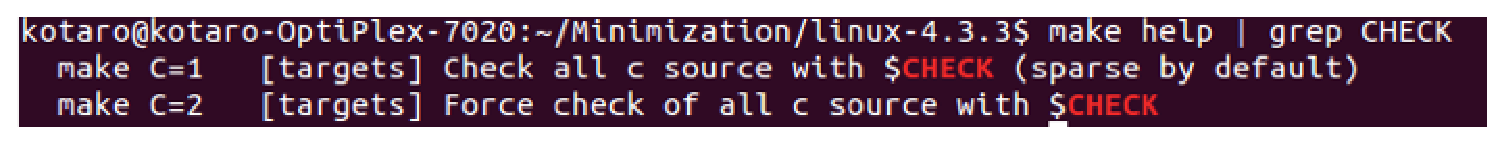
\includegraphics[width=\textwidth]{pic/check.eps}
  \caption{\acrshort{linux} KernelのMakefileで利用可能なソースコードチェック機能}
  \label{check}
\end{figure}
\par
\verb|CHECK| 変数で指定したチェックツールに対するオプションは、同じく \verb|make| コマンド中の \verb|CF| 変数で与えることができる(図\ref{cf})。
\begin{figure}[ht]
  \centering
  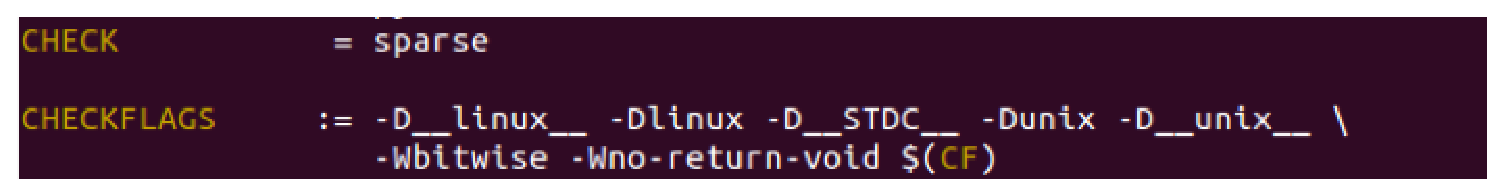
\includegraphics[width=\textwidth]{pic/cf.eps}
  \caption{\acrshort{linux} KernelのMakefile中で設定されているソースコードチェックツールとそのオプション}
  \label{cf}
\end{figure}
\par
\acrshort{codemini}の実装では、\acrshort{linux} Kernelの \verb|Makefile| に既に存在する図\ref{check}と図\ref{cf}の機能を利用して下記のようなコマンドで\acrshort{codemini}を実現する方針とした。
\begin{itembox}[l]{\acrshort{codemini}コマンド形式}
  \verb|make C=1 CHECK=minimize.py CF="-mindir ../minimized-tree"|
\end{itembox}
\par
\verb|minimize.py| は\acrshort{codemini}の\acrshort{py}スクリプトによる実装である。
\verb|CF| 変数で変換後のソースツリー生成場所を指定する。
これにより、通常のkernelビルドと同時に
各々のCソースファイルに対する\acrshort{codemini}が一括して実行される。
\verb|CHECK| 変数で指定したスクリプト \verb|minimize.py| には、各々のCソースファイルに対する \verb|gcc| コマンドと
同じオプション文字列が自動的に渡される。
そのため、\verb|CHECK| 変数を利用する方法は前述の\acrshort{overflow}の手順で必要だったビルドログの取得やgccコマンドの編集
といった中間処理が不要であり、全ての処理を1コマンドで完結できる利点がある。
\verb|minimize.py| スクリプト本体およびその詳しい使用手順は
\href{https://github.com/Hitachi-India-Pvt-Ltd-RD/minimization}{\acrshort{hub}のminimizationレポジトリで公開している} \cite{minimization}。
\subsubsection{\ref{enum:preprocess} プリプロセスコマンドの構築と実行}
以降は \verb|minimize.py| スクリプトの実装について処理の概要を記載する。
\par
\verb|minimize.py| は \verb|make| プロセスから呼ばれるとき、そのターゲットCファイルへの \verb|gcc| コマンドと同じオプション文字列を引数で受け取る。
\verb|minimize.py| は受け取ったオプション文字列の先頭に\verb|gcc -E -fdirectives-only | を追加した上で
その文字列をシステムコマンドとして実行する。
その結果、\verb|#ifdef| が消え、\verb|#include| が展開され、\verb|#define| がそのまま保存されたプリプロセス出力が得られる。
\subsubsection{\ref{enum:postprocess} 展開されたヘッダファイルの中身と余分な空白行の削除}
\verb|minimize.py| はプリプロセスの結果に対して \verb|#include| で展開されたヘッダファイルに該当する箇所を削除する。
\verb|gcc| のプリプロセス出力には以下のような形式で \verb|#include| の展開情報が残されており、これらは\textit{linemarkers}と呼ばれる。
プリプロセス出力からヘッダファイル展開箇所を特定するためには、\textit{linemarkers}を手掛かりとして用いる。
\begin{itemize}
  \item プリプロセス出力中の\textit{linemarkers}の例
  \begin{itemize}
    \item[] \verb|# 30 "/usr/include/sys/utsname.h" 2|
  \end{itemize}
\end{itemize}
\par
この\textit{linemarkers}の例は「この行以降のコードは \verb|/usr/include/sys/utsname.h| の30行目が展開されたもので、
かつ別の入れ子になった \verb|#include| の展開内容から返ってきた直後」であることを意味している。
\textit{linemarkers}の形式については以下のページが詳しい。 \\
 \href{https://gcc.gnu.org/onlinedocs/cpp/Preprocessor-Output.html}{Preprocessor Output - The C Preprocessor} \cite{linemarkers}
\par
\verb|minimize.py| は、\textit{linemarkers}を解析することで元のCファイルに存在しないヘッダファイルの展開内容を削除する。
その上で元のCファイルの内容と比較をして \verb|#include| 行の復元と、消えた \verb|#ifdef| ブロックに該当する空白行の削除を行う。
元のソースと最終的に得られるソースとの差分は無効な \verb|#ifdef| ブロックの削除のみであり、
\verb|#include| 行および \verb|#define| 行は元のまま保持される(図\ref{miniresult})。
\begin{figure}[ht]
  \centering
  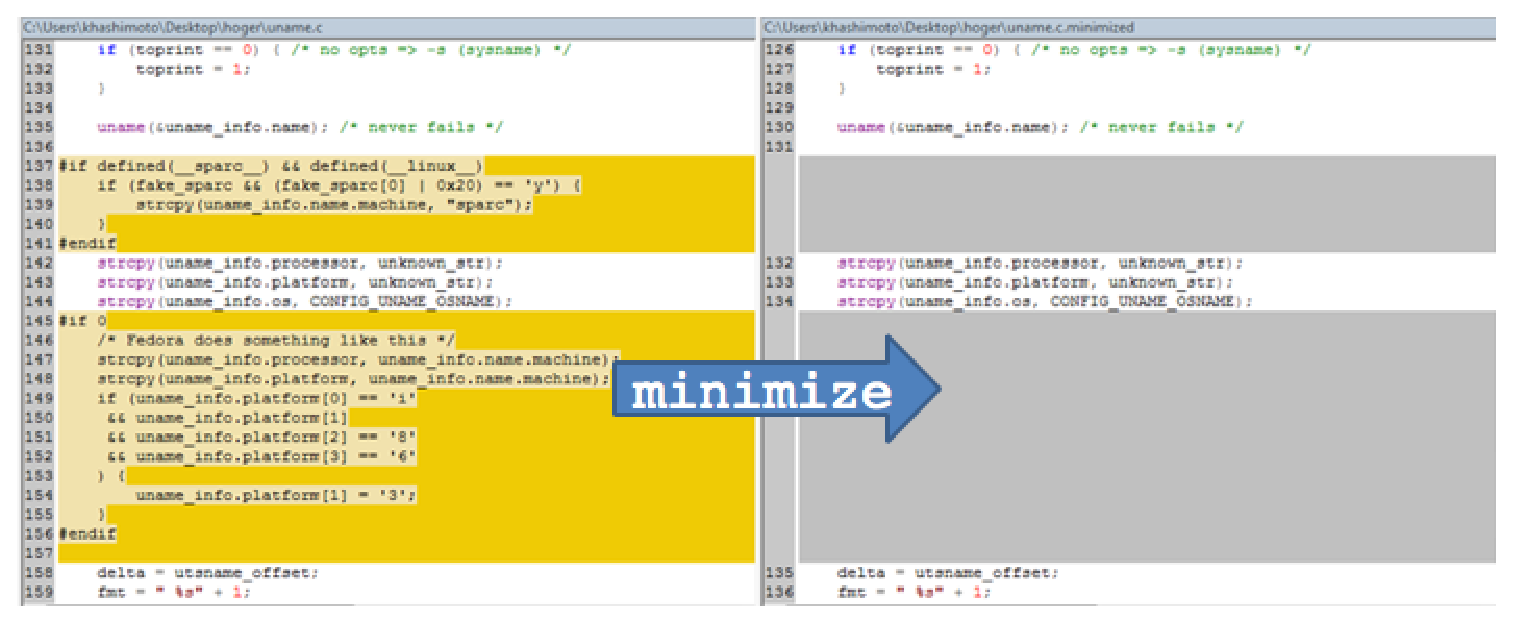
\includegraphics[width=\textwidth]{pic/miniresult.eps}
  \caption{\acrshort{codemini}の実行結果例}
  \label{miniresult}
\end{figure}
\par
\subsection{実行結果}
\verb|minimize.py| は当初\acrshort{linux} Kernelに対して適用することを想定して実装されたが、\verb|Makefile| 中の \verb|CHECK| 変数を利用する仕組みがそのまま
\acrshort{bb}にも適用できることが分かった。
\acrshort{linux} Kernelおよび\acrshort{bb}に対して \verb|minimize.py| を実行した結果削除されたソースコード量を表\ref{ministats}に示す。
ここでは実験対象として\acrshort{linux} Kernel 4.3.3と\acrshort{bb} 1.24.15を使用し、各々 \verb|allnoconfig| と \verb|defconfig| を適用したときの
\acrshort{codemini}結果を記載している。
実験はUbuntu 14.04 (x86\_64)で実施した。
\begin{table}[H]
  \caption{\acrshort{linux} Kernelと\acrshort{bb}への\acrshort{codemini}適用で削除されたコード量}
  \label{ministats}
  \centering
  \begin{tabular}{l|ll}
    設定 \textbackslash ターゲット & \acrshort{linux} Kernel 4.3.3 & \acrshort{bb} 1.24.15 \\
    \hline 
    \verb|defconfig| (x86) & 103144行(全体の5\%) & 20453行(全体の11\%)\\
    \verb|allnoconfig| & 64684行(全体の22\%) & 5945行(全体の34\%
%    \verb|defconfig| (x86) & \shortstack{103144行(全体の5\%) \\ $1804 / 2022$ファイルが処理対象} & \\
  \end{tabular}
\end{table}
\par
\acrshort{linux} Kernel、\acrshort{bb}ともに \verb|allnoconfig| 設定のときにコード削減割合が高い。
これは、無効化される機能が多くなるほど使用されない \verb|#ifdef| ブロックが増えることと対応している。
\par
\verb|minimize.py| 実行の結果生成されたソースツリーは素のソースツリーと同じ手順でビルドが可能であった。
ビルドの確認は、\acrshort{codemini}後のファイルとディレクトリをそのまま素のソースツリー上に上書きコピーして実施した。
これは\acrshort{codemini}生成物に \verb|Makefile| などのビルドに必要なスクリプト類が含まれないためである。
\par
\acrshort{codemini}は無効コードを削除するのみで、機能そのものには一切影響を与えてはいけない。
このことを確認するため、素のソースツリーのビルド生成物と\acrshort{codemini}で生成されたソースツリーのビルド生成物の比較を行うことを検討した。
各々ビルドの結果生成されたバイナリを \verb|objdump -d| コマンドで逆アセンブリしたところ、アセンブリコードの比較結果は表\ref{assemblycomp}のようになった。
\begin{table}[H]
  \caption{\acrshort{codemini}後のソースツリーによるビルド生成物と素のソースツリーによるビルド生成物とのアセンブリコード比較結果}
  \label{assemblycomp}
  \centering
  \begin{tabular}{l|ll}
    設定 \textbackslash ターゲットファイル & vmlinux.o & busybox(実行ファイル) \\
    \hline 
    \verb|defconfig| (x86) & 差分あり & 一致 \\
    \verb|allnoconfig| & 一致 & 一致
  \end{tabular}
\end{table}
\par
アセンブリコード( \verb|objdump -d| の出力)が一致するターゲットと設定の組み合わせに対してもバイナリファイルの直接比較結果は一致しない。
これはビルド生成物にビルドタイムスタンプ等の情報が埋め込まれていることが要因の一つである。
\verb|objdump -d| は実行ファイル中から実行部(executable section)のアセンブリコードを出力する。
表\ref{assemblycomp}において \verb|objdump -d| が一致することは、\verb|minimize.py| の処理内容が最終ビルド生成物の挙動に影響を与えないことを支持する。
しかし、\acrshort{linux} Kernelを\verb|defconfig| (x86)で\acrshort{codemini}適用した場合は、ビルド生成物のアセンブリコードと素のソースツリー由来のものとで差分があった。
この事象に対する調査、および \verb|minimize.py| がソフトウェアの機能そのものに一切影響を及ぼさないことの更なる検証方法検討は今後の課題である。
\par
\acrshort{linux} Kernelおよび\acrshort{bb}に対する\acrshort{codemini}実装は以下の\acrshort{hub}レポジトリで公開している(図\ref{minigithub})。\cite{minimization}
\begin{figure}[H]
%\begin{figure}[ht]
  \centering
  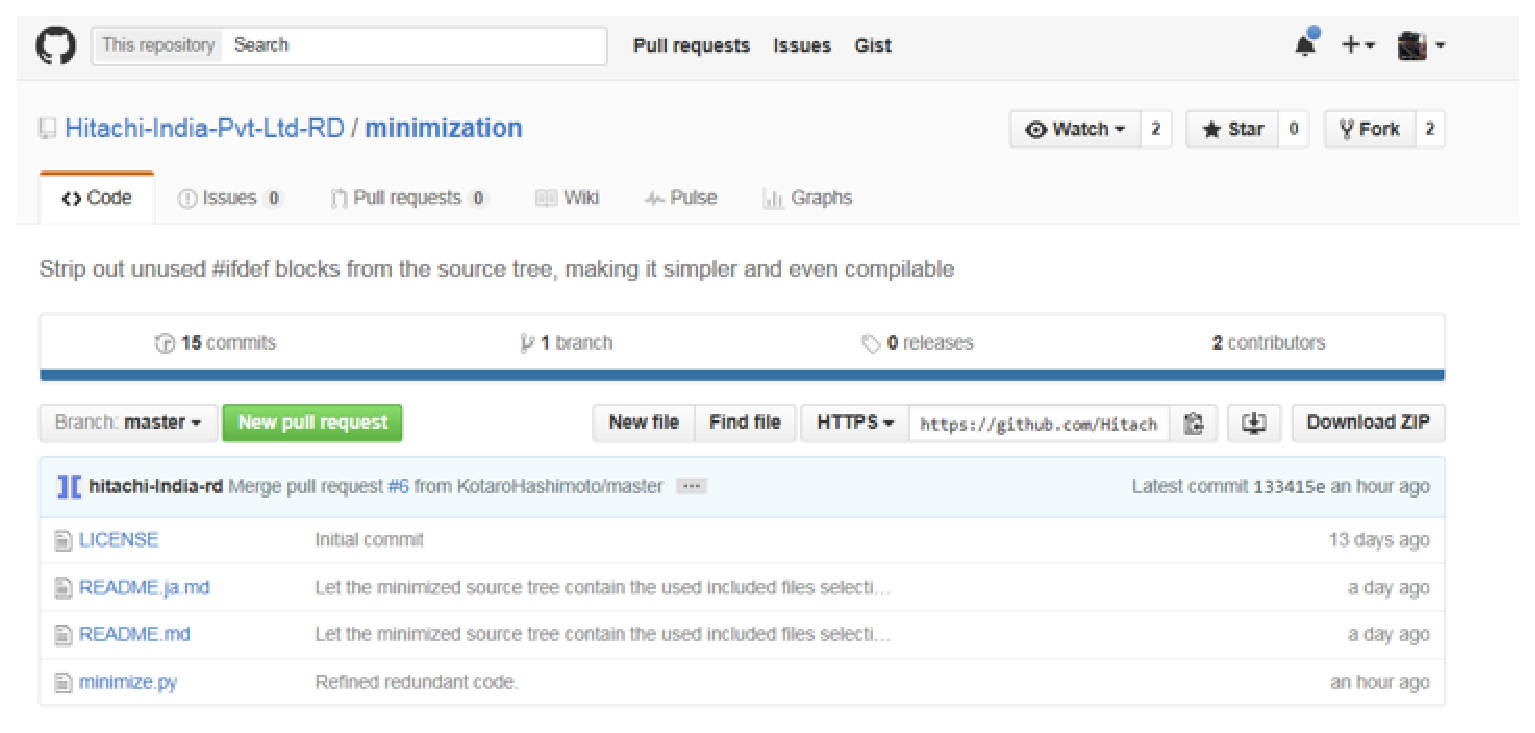
\includegraphics[width=\textwidth]{pic/minigithub.eps}
  \caption{\href{https://github.com/Hitachi-India-Pvt-Ltd-RD/minimization}{https://github.com/Hitachi-India-Pvt-Ltd-RD/minimization}}
  \label{minigithub}
\end{figure}
%\newline
\subsection{\acrshort{codemini}技法の利点と応用}
\acrshort{codemini}技法を適用することで、使用されないコードを削除することによるソースコードの可読性向上が期待される。
加えて、ソースコードのレビューや静的検証を行う際の検査対象範囲が限定される効果も考えられる。
本項では、可読性向上に関する評価と、検査対象範囲を限定することにより静的検証のパフォーマンスを向上させる応用例について記載する。
\subsubsection{変換後のソースコード複雑度評価}
\acrshort{codemini}適用によるソースコード可読性向上度合いを評価するため、ソースコードの複雑度を測定するツール
\href{https://www.gnu.org/software/complexity/manual/complexity.html}{\acrshort{comp}} \cite{comp}
を使用した。
\acrshort{comp}はCプログラムの複雑度を定量的に測定するために設計された\acrshort{gnu}ツールである。
コード複雑度の測定ツールとしては例えば\acrshort{mc}が知られている。
\acrshort{mc}は主に実行パス数に基づく情報からテストに必要な労力を数値化することを目的としているのに対して、
\acrshort{comp}はコードの長さや条件分岐の複雑さを評価することで、特に人間がコードを理解するための労力を数値化することを意図している。
\par
以下は、\acrshort{codemini}適用前の\acrshort{linux} Kernelソースツリー中のCソースファイルについて\acrshort{comp}で
複雑度を測定した結果である。
"Complexity Histogram"では、関数ごとに測定された複雑度スコアの分布($0 \sim 1999$)がコード行数の積算を度数として示されている。
複雑度スコアの平均値(Average line score)は23、中央値(50\%-ile score)は4、最大値(Highest score)は1846であった。
\begin{itembox}[l]{素の\acrshort{linux} Kernelソースツリーに対する\acrshort{comp}測定結果}
\small
\begin{verbatim}
$ find linux-4.4.1 -name "*.c" | xargs complexity -h
Complexity Histogram
Score-Range  Lin-Ct
    0-9      277794 ************************************************************
   10-19      49923 ***********
   20-29      17566 ****
   30-39       7189 **
   40-49       2148
   50-59       1961
   60-69        630
   70-79        563
   80-89        633
   90-99       1381

  100-199      5332 *
  200-299      2765 *
  300-399         0
  400-499         0
  500-599         0
  600-699         0
  700-799         0
  800-899         0
  900-999         0

 1000-1999     2345 *

Scored procedure ct:    18176
Non-comment line ct:   370230
Average line score:        23
25%-ile score:              2 (75% in higher score procs)
50%-ile score:              4 (half in higher score procs)
75%-ile score:              9 (25% in higher score procs)
Highest score:           1846 (setgamma() in linux-4.4.1/drivers/media/usb/gspca/topro.c)
\end{verbatim}
\end{itembox}
\par
次に、\verb|allnoconfig| 設定で\acrshort{codemini}適用した\acrshort{linux} Kernelソースツリーに対して複雑度を測定した結果を示す。
複雑度スコアの平均値(Average line score)は5、中央値(50\%-ile score)は2、最大値(Highest score)は158であった。
なお、\acrshort{codemini}適用前の測定結果で複雑度スコアが最大であった関数 \verb|setgamma() (linux-4.4.1/drivers/media/usb/gspca/topro.c)|
は\acrshort{codemini}適用後のソースツリーに含まれていなかった。
\begin{itembox}[l]{allnoconfig 設定の\acrshort{linux} Kernelソースツリーに対する\acrshort{comp}測定結果}
\small
\begin{verbatim}
$ find minimized-tree -name "*.c" | xargs complexity -h
Complexity Histogram
Score-Range  Lin-Ct
    0-9       85190 ************************************************************
   10-19       7640 *****
   20-29       1004 *
   30-39        944 *
   40-49        102
   50-59        109
   60-69         96
   70-79          0
   80-89          0
   90-99          0

  100-199       396

Scored procedure ct:     7870
Non-comment line ct:    95481
Average line score:         5
25%-ile score:              1 (75% in higher score procs)
50%-ile score:              2 (half in higher score procs)
75%-ile score:              5 (25% in higher score procs)
Highest score:            158 (zlib_inflate() in minikern/lib/zlib_inflate/inflate.c)
Unscored procedures:        4
\end{verbatim}
\end{itembox}
\par
続いて、\verb|defconfig| (x86)設定で\acrshort{codemini}適用した\acrshort{linux} Kernelソースツリーに対して複雑度を測定した結果を示す。
複雑度スコアの平均値(Average line score)は7、中央値(50\%-ile score)は3、最大値(Highest score)は194であった。
\begin{itembox}[l]{defconfig(x86)設定の\acrshort{linux} Kernelソースツリーに対する\acrshort{comp}測定結果}
\small
\begin{verbatim}
$ find minimized-tree -name "*.c" | xargs complexity -h
Complexity Histogram
Score-Range  Lin-Ct
    0-9      675258 ************************************************************
   10-19      86562 ********
   20-29      27818 **
   30-39      12037 *
   40-49       5734 *
   50-59       2583
   60-69       3124
   70-79       3047
   80-89        281
   90-99       1051

  100-199      2135

Scored procedure ct:    50155
Non-comment line ct:   819630
Average line score:         7
25%-ile score:              2 (75% in higher score procs)
50%-ile score:              3 (half in higher score procs)
75%-ile score:              7 (25% in higher score procs)
Highest score:            194 (inflate_fast() in minikern/lib/zlib_inflate/inffast.c)
Unscored procedures:        9
\end{verbatim}
\end{itembox}
\par
以上を総合すると、複雑度スコアの平均値、中央値、最大値はいずれも \verb|allnoconfig| $<$ \verb|defconfig| $<$ (\acrshort{codemini}非適用) の関係となり、
\acrshort{codemini}によって削除されたコード量の大小と対応する結果が得られた(表\ref{kcomp})。
\begin{table}[H]
  \caption{\acrshort{linux} Kernelソースツリーの\acrshort{codemini}適用前後に対する\acrshort{comp}スコア測定結果}
  \label{kcomp}
  \centering
  \begin{tabular}{l|lll}
    \normalsize{スコア種類 \textbackslash 設定条件} & \verb|allnoconfig| & \verb|defconfig| (x86) & \acrshort{codemini}非適用 \\
    \hline 
    平均値(Average line score) & 5 & 7 & 23 \\
       (25\%-ile score) & 1 & 2 & 2 \\
    中央値(50\%-ile score) & 2 & 3 & 4 \\
       (75\%-ile score) & 5 & 7 & 9 \\
    最大値(Highest score) & 158 & 194 & 1846
  \end{tabular}
\end{table}
\par
同様の複雑度測定評価を\acrshort{bb}に対して行った結果を表\ref{bcomp}に示す。
\acrshort{bb}での測定結果においても\acrshort{linux} Kernelと同様に概ね \verb|allnoconfig| $<$ \verb|defconfig| $<$ (\acrshort{codemini}非適用) の関係が得られた。
\begin{table}[H]
  \caption{\acrshort{bb}ソースツリーの\acrshort{codemini}適用前後に対する\acrshort{comp}スコア測定結果}
  \label{bcomp}
  \centering
  \begin{tabular}{l|lll}
    \normalsize{スコア種類 \textbackslash 設定条件} & \verb|allnoconfig| & \verb|defconfig| (x86) & \acrshort{codemini}非適用 \\
    \hline 
    平均値(Average line score) & 19 & 21 & 22 \\
       (25\%-ile score) & 2 & 3 & 3 \\
    中央値(50\%-ile score) & 5 & 9 & 9 \\
       (75\%-ile score) & 21 & 24 & 25 \\
    最大値(Highest score) & 283 & 283 & 283
  \end{tabular}
\end{table}
\par
以上から、\acrshort{codemini}で無効コードを削除した結果では
\acrshort{comp}ツールによる客観的な指標においてソースコードの可読性が向上することが示された。
\subsubsection{検査対象範囲の最小化}
\label{minigraph}
本項では、\acrshort{codemini}がソースコードの検査対象範囲を限定する効果に着目し、
その性質を応用することで静的検証におけるパフォーマンスを向上させることができる例を示す。
\par
テストカバレッジ測定の原理を考えたとき、一般にテストカバレッジは
テスト実施した行数($LOC_{exercised}$)の総コード行数($LOC_{total}$)に対する比で表される(式(\ref{usocov}))。
\begin{equation}
  TestCoverage = \frac{LOC_{exercised}}{LOC_{total}}
\label{usocov}
\end{equation}
\par
ここで、コンパイル対象とならない無効な \verb|#ifdef| コードブロックがソースコードに含まれる場合は
無効なコードブロック行数$LOC_{unused}$を$LOC_{total}$から引くことでより正確なカバレッジが測定できる(式(\ref{minicov}))。
\begin{equation}
  TestCoverage = \frac{LOC_{exercised}}{LOC_{total} - LOC_{unused}}
\label{minicov}
\end{equation}
\par
式(\ref{minicov})は、使用されないコードを多く特定するほど計算上テストカバレッジが向上する(より正確なカバレッジ評価となる)ことを意味する。
使用されないコードが特定されない限り、$LOC_{exercised}$を増やすためにどれだけテストに労力を費やしたとしても
達成できるカバレッジは100\%未満($1 - \frac{LOC_{unused}}{LOC_{total}}$)で制限される(図\ref{coveragesagi})。
ここで\acrshort{codemini}適用により$LOC_{unused}$を明らかにすることができれば、
達成し得るテストカバレッジをその分向上させることができる。
このように、\acrshort{codemini}は検査範囲を最小化する効果がある。
この技法を"minimization"と呼ぶことはこの意味での「最小化」の効果が得られることに由来する。
\begin{figure}[ht]
  \centering
  \includegraphics[width=\textwidth]{pic/coveragesagi.eps}
  \caption{\acrshort{codemini}適用により正確なテストカバレッジ測定が可能となる}
  \label{coveragesagi}
\end{figure}
%\paragraph{関数コールグラフを枝刈りする応用例}\mbox{}\\
\subsubsection{関数コールグラフを枝刈りする応用例}
\acrshort{codemini}で予めソースコードを最小化することで関数コールグラフの解析が簡単になる例を示す。
\ref{callgraph}項で述べたように、関数コールグラフはトレーサと組合わせてパスカバレッジを測定する目的で使用できる。
関数コールグラフ導出により実行され得る全関数呼び出しパスを特定することは、式(\ref{minicov})において分母($LOC_{total} - LOC_{unused}$)に相当にする箇所を測定することに対応する。
\par
ここでは\acrshort{cflow}を使用して\acrshort{bb}の \verb|init_main() (init/init.c)| に対する関数コールグラフを生成する。
グラフ画像生成は次のコマンドで実施した。
\begin{itemize}
  \item \acrshort{cflow}で\acrshort{bb}から \verb|init_main()| の関数コールグラフを生成する手順
  \begin{itemize}
    \item[] \verb!$ cd busybox-1.24.1!
    \item[] \verb!$ cflow -d 5 -b init/init.c | tree2dotx | dot -Tsvg -o init.svg!
  \end{itemize}
\end{itemize}
\par
\acrshort{codemini}適用前の関数コールグラフを図\ref{orggraph}に示す。
このグラフは \verb|#ifdef| ブロックで無効化される関数も含まれているため複雑で非常に見通しが悪い。
\acrshort{codemini}適用前グラフのノード数は94、エッジ数は140であった。
図\ref{minigraph}は\acrshort{codemini}適用後の関数コールグラフである。
こちらのグラフはコンパイル対象である関数のみが含まれるため複雑さが改善している。
\acrshort{codemini}適用後のグラフのノード数は85、エッジ数は123であった。
\begin{figure}[ht]
 \begin{minipage}{0.53\hsize}
  \begin{center}
   \includegraphics[width=\textwidth]{pic/orggraph.eps}
  \end{center}
  \caption{適用前(94ノード、140エッジ)}
  \label{orggraph}
 \end{minipage}
 \begin{minipage}{0.47\hsize}
  \begin{center}
   \includegraphics[width=\textwidth]{pic/minigraph.eps}
  \end{center}
  \caption{適用後(85ノード、123エッジ)}
  \label{minigraph}
 \end{minipage}
 \caption{\acrshort{codemini}適用前後の関数コールグラフサイズ比較}
\end{figure}
\par
以上の結果から、関数コールグラフ解析において事前に\acrshort{codemini}を実施することで
グラフのサイズを最小化することができ、解析の効率向上やカバレッジ向上等の効果を期待できることが分かる。
ちなみに \verb|cflow| コマンド自体にもプリプロセスオプションが備わっているため、\acrshort{codemini}を使用しなくとも
コンパイル対象外の関数をグラフに含めないことは可能である。
ただし、\verb|cflow| コマンドでプリプロセスを行う場合は \verb|gcc| コンパイルオプション文字列をビルドログから取得して
\verb|cflow| の \verb|--cpp| オプションで渡す作業を各Cファイルについて行わなければならず、手間がかかる上に誤りが発生しやすい。
それに対して \verb|minimize.py| は1コマンドで一括して全てのCファイルに対するプリプロセスを行うことができる利点がある。
\par
\acrshort{cflow}に限らず、\acrshort{cocci}や\acrshort{cpa}等の各種検証ツールもそれぞれプリプロセスオプションが備わっていることが多い。
ただし、各検証ツールはプリプロセス自体が主目的ではないためそれらのプリプロセス処理は \verb|gcc| のものと比べて完全でないことが多く、
中には独自のプリプロセス挙動を示すものもある。
\verb|minimize.py| は変換後のソースツリーも元と同じ手順でビルド可能であることを保証するものであり、
これは\acrshort{codemini}技法が特定の検証ツールに依存せず一般に様々な検証技法の前処理として応用できることを示唆する。
\subsubsection{部分ソースツリーの抽出}
\verb|minimize.py| は \verb|Makefile| がサポートするサブターゲットに対しても作用する。
\verb|minimize.py| を実行する \verb|make|コマンドでサブターゲットを指定した場合、
そのサブターゲットが依存するソースファイルのみを含む部分ツリーが抽出される。
抽出された部分ツリー中のCソースファイルは\acrshort{codemini}適用後の状態となる。
以下は、\acrshort{bb}の \verb|init| サブターゲットから依存されるソースファイルを、
コンパイル対象のコードブロックのみを含む形で部分的に抽出するコマンド例である。
\begin{itemize}
  \item \acrshort{bb}の \verb|init| サブターゲットで使われるソースファイルとコードのみを抽出するコマンド例
  \begin{itemize}
    \item[] \verb!$ cd busybox-1.24.1!
    \item[] \verb!$ make init C=2 CHECK=minimize.py CF="-mindir ../min-init"!
  \end{itemize}
\end{itemize}
\par
上記コマンドの実行結果抽出された部分ソースツリーは図\ref{subtarget}のようになる。
\begin{figure}[ht]
  \centering
  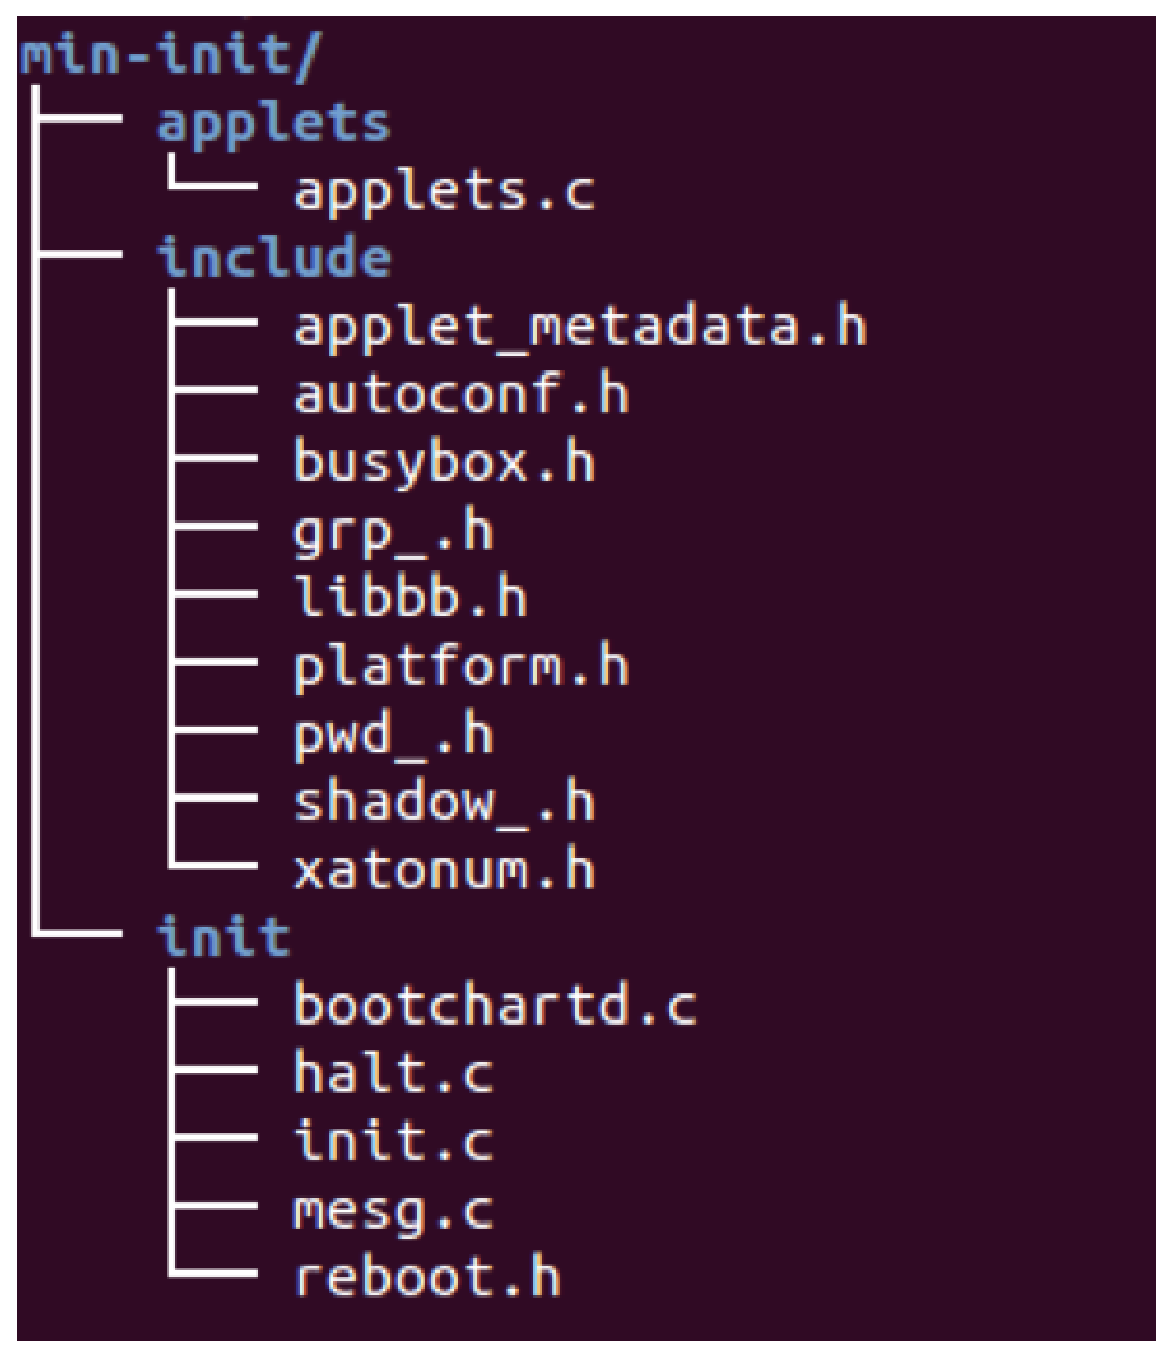
\includegraphics[width=0.4\textwidth]{pic/subtarget.eps}
  \caption{\acrshort{bb}のinitサブターゲット対象に\acrshort{codemini}適用して得られた部分ツリー}
  \label{subtarget}
\end{figure}
\par
指定したサブターゲットからどのファイルが実際にコンパイル対象として使われているかが明らかになることで、
例えばコードレビューの効率が向上する効果が期待される。
\subsection{まとめと今後の課題}
\acrshort{codemini}技法はソースコードの可読性を向上させる効果がある。
この性質はコードレビューやデバッグ効率向上のために利用できる。
また、\acrshort{codemini}技法は検査対象範囲を限定する効果がある。
これは図\ref{100} (\acrshort{iec61508}-3 Table B.2 - Dynamic analysis and testing)において
各種カバレッジ100\%を達成するために有力な手段となる。
または、テストを実施しない箇所がコンパイル対象外であることに示すエビデンスとして\acrshort{codemini}の結果を利用することも考えられる。
使用されないコードを特定し検査対象から除外することは、検証ツールが生成する\acrshort{fp}絶対量を抑制する結果にもつながる。
さらに、全体のコード量が削減されることで静的検証に要する時間と計算資源コストを節約できる。
Nicholas Mc Guire(\acrshort{ot})の実験によると、3時間要していた\acrshort{cocci}実行が\acrshort{codemini}適用後のソースツリーでは15分程度に短縮されたという。
\par
現状 \verb|minimize.py| がサポートするターゲットは\acrshort{linux} Kernelと\acrshort{bb}で、変換後ソースツリーのビルドを確認した設定は \verb|allnoconfig|、\verb|defconfig| (x86)、および \verb|omap2plus_defconfig|(ARMターゲットへのクロスビルド)である。
今後はさらに適用できるターゲットと設定を拡充していく予定である。
また\acrshort{codemini}適用後のソースツリーが素のソースツリーと機能的に等価であることの検証が未解決課題である。
\par
\acrshort{codemini}は一般に検証ツール・手法のパフォーマンスを増強させる技法であるため、組み合わせによって様々な使い方の可能性がある。
今後多数の\acrshort{codemini}技法の応用方法を考案し、\acrshort{sil2linuxmp}コミュニティに提案を行っていく方針である。
